\chapter{Measures}

InVesalius allows linear and angular measurements in 2D (axial, coronal and sagittal planes) and 3D (surfaces). It is also possible to take measurements volume and area on surfaces.

\section{Linear Measurement}

%Para realizar medições lineares, é necessário ativar o recurso clicando no atalho
%correspondente localizado na barra de ferramentas (figura \ref{fig:measure_line_original}).

To perform linear measurements, it is necessary to activate the feature by clicking on the shortcut corresponding toolbar located (figure\ref{fig:measure_line_original}).

\begin{figure}[!htb]
\centering

\includegraphics[scale=0.2]{measure_line_original}
\caption{Shortcut to activate linear measurement}
\label{fig:measure_line_original}
\end{figure}

%Uma medição linear é definida entre dois pontos. Com o recurso ativado, clique
%\textbf{uma} vez sobre a imagem para estabelecer o ponto inicial. Em seguida,
%posicione o ponteiro do mouse no ponto final e clique \textbf{uma} vez novamente.
%A medição é executada e o resultado é exibido automaticamente sobre a imagem ou
%superfície.

A linear measurement is defined between two points. With the feature enabled, click \textbf{once} on the image to set the starting point. Then position the mouse pointer on the end point and click \textbf{one} again. The measurement is performed and the result is automatically displayed on the image or surface.

%A figura \ref{fig:axial_linear} mostra uma medida linear em 2D na orientação axial, e a figura \ref{fig:3d_linear} mostra outra medida linear em 3D (superfície).

The figure \ref{fig:axial_linear} shows a 2D linear measure in the axial orientation, and the figure \ref{fig:3d_linear} shows another linear measure in 3D (surface).

%Uma vez feita a medida linear em 2D, é possível edita-la, para isso é necessário posicionar o mouse sobre uma das extremidades, manter o \textbf{botão direito do mouse} pressionado e arrastar para a posição desejada.

Once you have made the 2D linear measurement, you can edit it by placing the mouse on one end, holding down the \textbf{right mouse button} and dragging it to the desired position.

\begin{figure}[!htb]
\centering
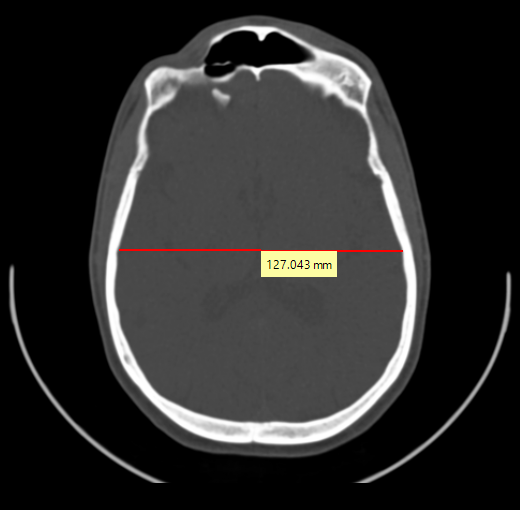
\includegraphics[scale=0.4]{axial_linear.png}
\caption{Linear measure on image}
\label{fig:axial_linear}
\end{figure}

\begin{figure}[!htb]
\centering
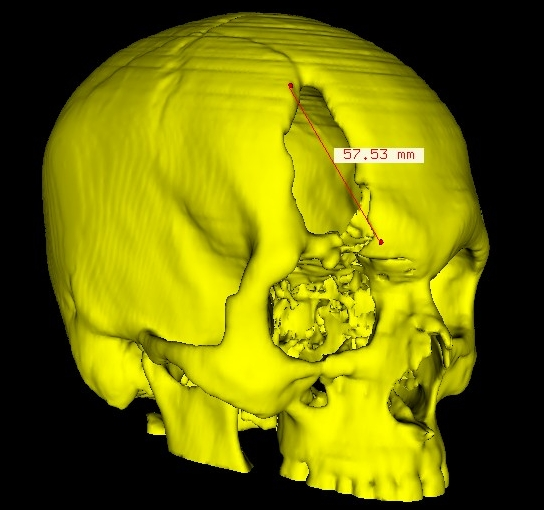
\includegraphics[scale=0.3]{3d_linear.jpg}
\caption{Linear measure on surface}
\label{fig:3d_linear}
\end{figure}

\textbf{Note: The linear measurement is given in millimeters (mm).}

\section{Angular Measurement}

%Uma medição angular em 2D ou sobre uma superfície (3D) pode ser realizada clicando-se
%no atalho ilustrado na figura \ref{fig:atalho_angular}.

An angular measurement in 2D on a surface (3D) can be done by clicking on the shortcut shown in figure~\ref{fig:atalho_angular}.

\begin{figure}[!htb]
\centering

\includegraphics[scale=0.2]{measure_angle_original}
\caption{Shortcut for angle measurement}
\label{fig:atalho_angular}
\end{figure}

%Para efetuar a medição angular, é necessário fornecer os três pontos que descreverão o
%ângulo a ser medido, A\^{B}C. Posicione o ponteiro do mouse e clique \textbf{uma} vez
%com o botão esquerdo para determinar o primeiro ponto, A. Para inserir o segundo ponto,
%B (o vértice do ângulo ou o "centro do transferidor"), posicione o ponteiro do mouse e
%clique \textbf{uma} vez novamente. Repita as mesmas ações para determinar o terceiro
%ponto, C. A medição é executada e, automaticamente, a medida resultante é exibida sobre
%a imagem ou superfície.

To perform the angular measurement, is necessary to provide the three points that will describe the angle to be measured, A\^{B}C. Click \textbf{one} instead with the left button to determine the first point, A. To insert the second point, B (the vertex of the angle or the "center"), position the mouse pointer and click \textbf{one} again. Repeat the same actions to determine the third point, C. The resulting measurement is displayed on the image or surface.

%A figura \ref{fig:axial_angular} ilustra uma medida angular em uma imagem plana, e a figura \ref{fig:axial_superficie} ilustra uma medida angular sobre uma superfície.

The figure \ref{fig:axial_angular} illustrates an angular measurement on a flat image, and the figure \ref{fig:axial_superficie} illustrates an angular measurement on a surface.

%A exemplo da medida linear em 2D, também é possível editar a medida angular 2D, para isso é necessário posicionar o mouse sobre uma das extremidades, manter o \textbf{botão direito do mouse} pressionado e arrastar para a posição desejada.

As 2D linear measurement, you can also edit the 2D angular measurement, so you need to position the mouse on one end, hold down the \textbf{right mouse button} and drag it to the desired position.

\begin{figure}[!htb]
\centering
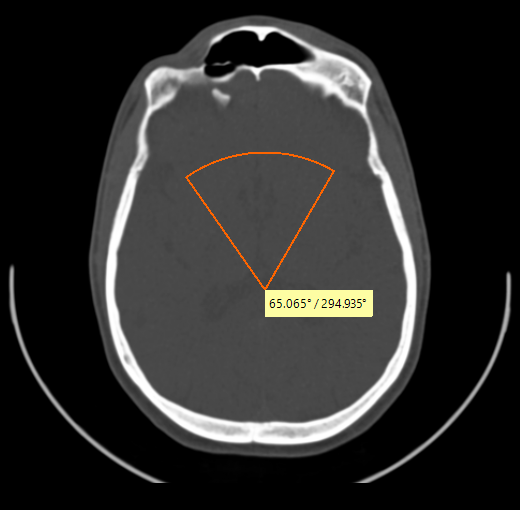
\includegraphics[scale=0.38]{axial_angular.png}
\caption{Angular measurement}
\label{fig:axial_angular}
\end{figure}

\begin{figure}[!htb]
\centering
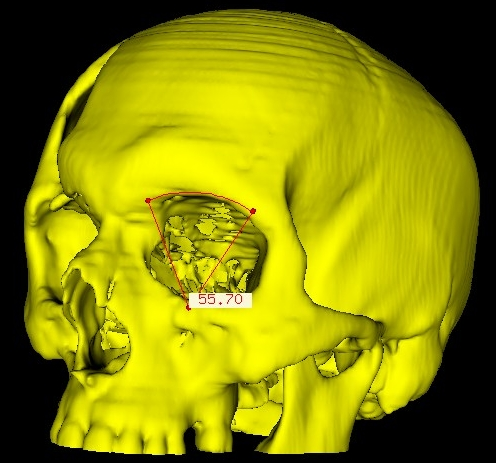
\includegraphics[scale=0.33]{angular_superficie.jpg}
\caption{Angular measurement on surface}
\label{fig:axial_superficie}
\end{figure}

\textbf{Note: Angular measurement is shown in degrees ($^{\circ}$)}


\section{Volumetric Measurement}

%As medições de volume e área são feitas automaticamente ao se criar uma nova superfície.
%Elas são exibidas na aba \textbf{Superfícies 3D}, no painel de gerenciamento de \textbf{Dados}, localizado no canto
%inferior esquerdo da tela, como ilustra a figura \ref{fig:volumetric_mensure}.

Volume and area measurements are made automatically when you create a new surface. they are displayed in the \textbf{Surfaces 3D} tab in the \textbf{Data} management panel, located in the corner
Bottom left of the screen, as illustrated in figure~\ref{fig:volumetric_mensure}.

\begin{figure}[!htb]
\centering
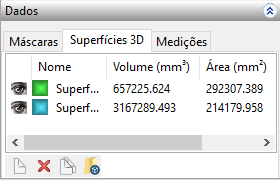
\includegraphics[scale=0.7]{painel_volumetric_measures_pt.png}
\caption{Volumetric measurements}
\label{fig:volumetric_mensure}
\end{figure}

\textbf{Note: Volume measurement is given in cubic millimeter ($mm^3$), already the one of area in square millimeter ($mm^2$)}
